\documentclass{article}
\usepackage{tikz}
\usetikzlibrary{arrows.meta}

\begin{document}

\begin{figure}[h]
    \centering
    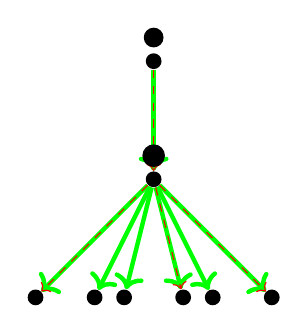
\begin{tikzpicture}[scale=1.5, every node/.style={circle, fill, inner sep=0pt, minimum size=2mm}]
        % Nodes
        \node (x) at (0, 1) {};
        \node (y) at (0, 0) {};
        \node (a) at (-1, -1) {};
        \node (b) at (-0.5, -1) {};
        \node (c) at (-0.25, -1) {};
        \node (d) at (0.25, -1) {};
        \node (e) at (0.5, -1) {};
        \node (f) at (1, -1) {};
        
        % Edges
        \draw[->, ultra thick, green] (x) -- (y);
        \draw[->, ultra thick, green] (y) -- (a);
        \draw[->, ultra thick, green] (y) -- (b);
        \draw[->, ultra thick, green] (y) -- (c);
        \draw[->, ultra thick, green] (y) -- (d);
        \draw[->, ultra thick, green] (y) -- (e);
        \draw[->, ultra thick, green] (y) -- (f);
        
        \draw[->, dashed, red] (x) -- (y);
        \draw[->, dashed, red] (y) -- (a);
        \draw[->, dashed, red] (y) -- (d);
        \draw[->, dashed, red] (y) -- (f);
        
        % Labels
        \node at (0, 1.2) {$x$};
        \node at (0, 0.2) {$y$};
    \end{tikzpicture}
    \caption{An illustration of a $(k,3)$-decomposition $(F_k,F_3)$ of a long $(k,3)$-out-forcer for some $k\geq 4$. The dashed red arcs are in $A(F_3)$ and the solid green arcs are in $A(F_k)$.}
    \label{fig:k3_decomposition}
\end{figure}

\end{document}